\section{Modelo de dominio}\label{cap:modelo_de_dominio}

En esta sección se detalla el diseño conceptual del sistema, incluyendo las entidades clave y sus relaciones. El modelo refleja la estructura lógica del dominio de la Semana Santa, garantizando una representación fiel de sus procesos, actores y reglas de negocio. Tras las correcciones indicadas por el tutor sobre la versión anterior del diagrama, y una segunda ronda de ajustes propios, se explican a continuación con más detalle las abstracciones incluidas en la Figura~\ref{fig:DiagramDomain}, la relación entre ellas y las decisiones de diseño tomadas para resolver los puntos que generaban confusión.

\clearpage
\begin{figure}[H]
\centering
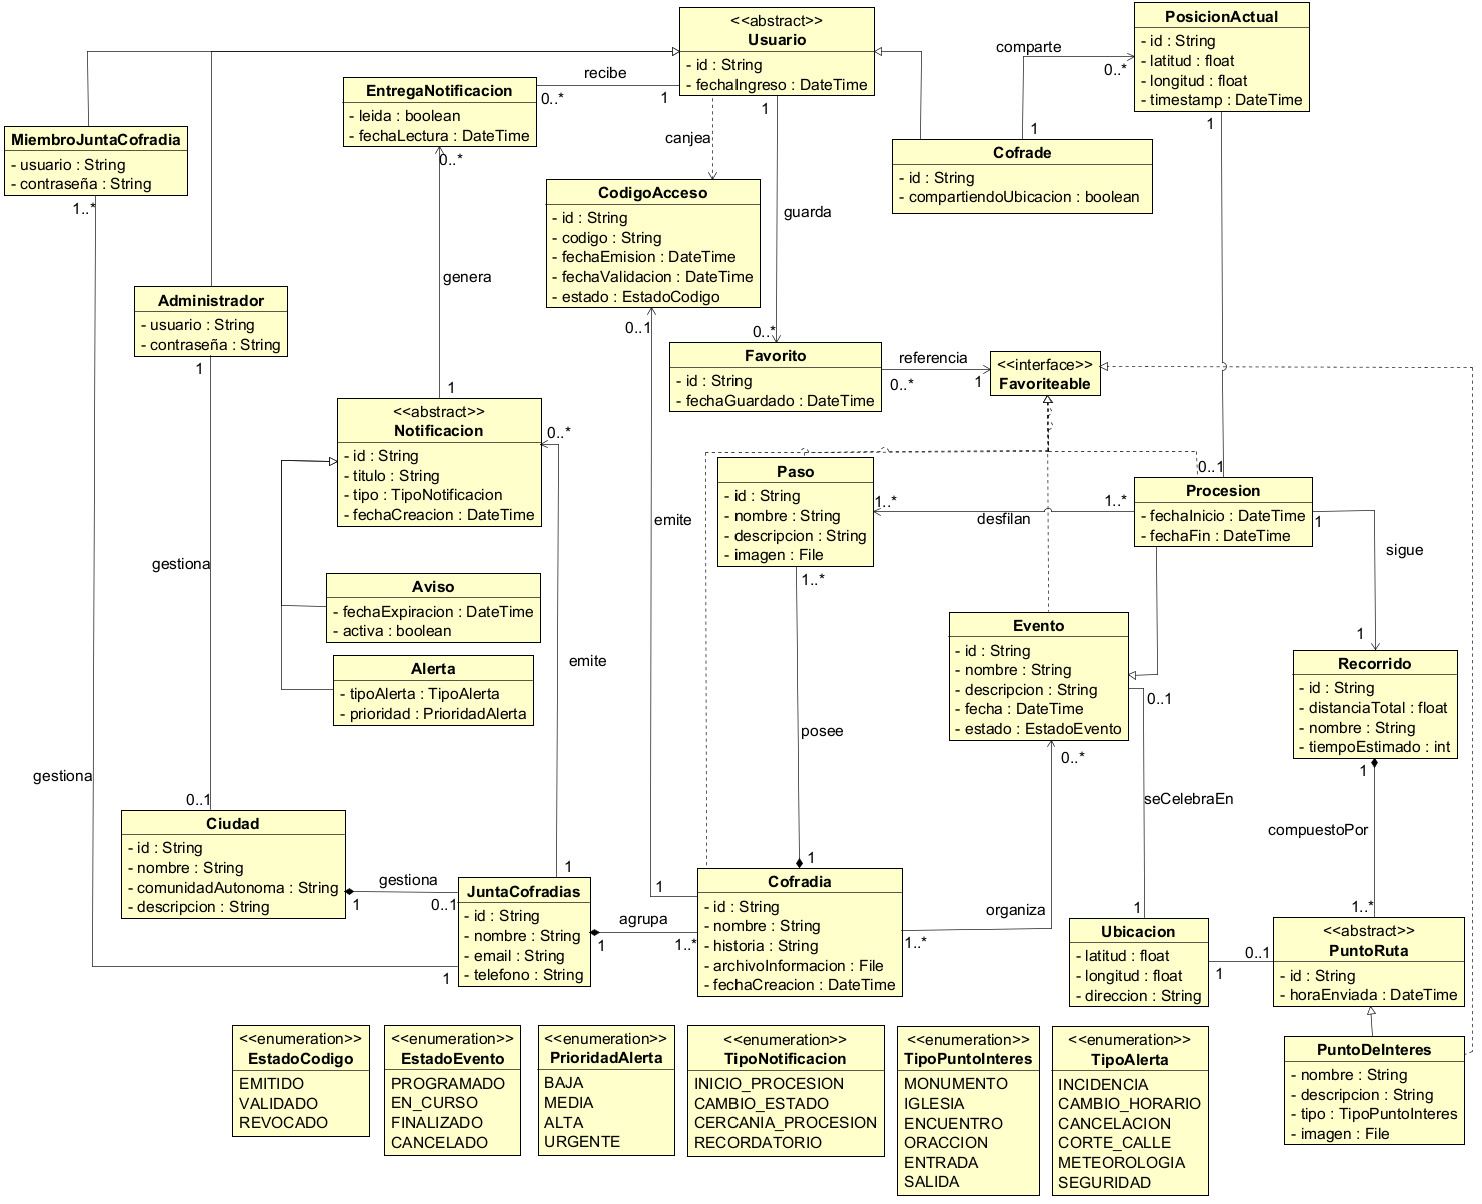
\includegraphics[width=1\textwidth,height=0.85\textheight,keepaspectratio]{imagenes/DiagramaDeDominio.png}
\caption{Diagrama de dominio del proyecto}
\label{fig:DiagramDomain}
\end{figure}

\subsection{Usuarios y roles}

En la versión anterior, todas las asociaciones relativas al usuario (compartir ubicación, guardar favoritos, canjear un código de acceso...) partían de una única clase \texttt{Usuario}, lo que generaba confusión porque algunas de esas asociaciones sólo tienen sentido para un cofrade. Para eliminarla, \texttt{Usuario} pasa a ser una clase abstracta con lo común a cualquier persona que usa la aplicación sin necesidad de registro (\texttt{id} y \texttt{fechaIngreso}, guardar \texttt{Favorito} y recibir \texttt{EntregaNotificacion}), de la que \texttt{Cofrade} hereda añadiendo \texttt{compartiendoUbicacion} y la posibilidad de compartir su \texttt{PosicionActual}.

\texttt{Administrador} y \texttt{MiembroJuntaCofradia} se modelan como clases independientes, al margen de la jerarquía de \texttt{Usuario}: ambas representan cuentas de acceso a paneles de gestión (con su propio \texttt{usuario} y \texttt{contraseña}), y no perfiles de la aplicación pública, por lo que su forma de autenticarse no tiene relación con la de un ciudadano o un cofrade. \texttt{Administrador} administra las \texttt{Ciudad} y las \texttt{JuntaCofradias} del sistema (RF-26 y RF-34); \texttt{MiembroJuntaCofradia} es quien, en representación de una \texttt{JuntaCofradias}, gestiona su contenido (cofradías, eventos, procesiones, alertas...), ya que la propia \texttt{JuntaCofradias} es una entidad organizativa y no una persona que inicia sesión.

El canje de un \texttt{CodigoAcceso} se modela como una dependencia de \texttt{Usuario} hacia \texttt{CodigoAcceso} (\textit{canjea}) y no como una asociación permanente: representa la acción de introducir el código, tras la cual, si es válido, el usuario pasa a ser un \texttt{Cofrade}. El resultado de esa acción queda registrado en el propio \texttt{CodigoAcceso}, a través de su \texttt{estado} (\texttt{EstadoCodigo}: emitido, validado o revocado) y su \texttt{fechaValidacion}.

\subsection{Ciudad y Junta de Cofradías}

Una \texttt{Ciudad} está gestionada como máximo por una \texttt{JuntaCofradias} (multiplicidad \texttt{0..1}), y no por varias: en el dominio de la aplicación cada ciudad cuenta con una única junta de cofradías de referencia (RI-10), que agrupa a su vez todas las \texttt{Cofradia} de esa localidad (\texttt{1..*}) y cuenta con uno o varios \texttt{MiembroJuntaCofradia} que la gestionan desde el panel correspondiente.

\subsection{Cofradías, eventos y procesiones}

Cada \texttt{Cofradia} posee uno o varios \texttt{Paso} (relación de composición, ya que un paso no existe sin la cofradía a la que pertenece) y organiza uno o varios \texttt{Evento}. La relación \textit{organiza} es de muchos a muchos: un mismo evento puede estar organizado conjuntamente por varias cofradías (por ejemplo, una procesión general o un acto conjunto de Semana Santa en el que participan distintas hermandades), y no únicamente por una.

Un \texttt{Paso} puede desfilar en más de una \texttt{Procesion} (por ejemplo, en la procesión propia de su cofradía y en una procesión conjunta como una general o un vía crucis), de ahí que la relación \textit{desfilan} sea de muchos a muchos. Cada \texttt{Procesion} está vinculada a un \texttt{Evento} y sigue un \texttt{Recorrido} (\textit{sigue}), compuesto a su vez por distintos \texttt{PuntoRuta}, clase abstracta de la que heredan \texttt{Ubicacion} y \texttt{PuntoDeInteres}.

La \texttt{Procesion} no incorpora un atributo propio de descripción: su información descriptiva se obtiene a través del \texttt{Evento} al que está vinculada (que sí tiene \texttt{descripcion}) y de la \texttt{historia} de la \texttt{Cofradia} que lo organiza, evitando así duplicar el mismo dato en dos sitios. Por su parte, \texttt{Evento} se asocia a una \texttt{Ubicacion} (\textit{seCelebraEn}) que recoge la latitud, longitud y dirección donde tiene lugar (un pregón, un traslado, un concierto...), reutilizando la misma clase que ya se emplea para los puntos de un recorrido, en lugar de duplicar un atributo de dirección suelto.

Por coherencia con el resto de elementos que pueden marcarse como favoritos, la interfaz \texttt{Favoriteable} la realizan \texttt{Evento}, \texttt{Procesion} y \texttt{Cofradia}, que son los tres tipos de elemento que un usuario puede marcar como favorito según el requisito RF-12.

\subsection{Geolocalización en tiempo real}

Para la geolocalización en tiempo real, un \texttt{Cofrade} puede compartir su posición durante una procesión, lo que genera instancias de \texttt{PosicionActual}. A partir de las distintas posiciones compartidas por los cofrades que participan en una misma procesión, el backend calcula una única \texttt{PosicionActual} agregada, que es la que queda asociada a la \texttt{Procesion} como su posición en vivo (\textit{procesionEnVivo}) y la que consultan el resto de usuarios de la aplicación. Es decir, de cara al usuario que sigue la procesión, ésta se representa como un único punto (el resultado del cálculo), y no como el conjunto de puntos individuales de cada cofrade ni como un trazo continuo; esta decisión de diseño quedará confirmada con el resto del equipo antes de la implementación.

\subsection{Notificaciones, avisos y alertas}

La comunicación con los usuarios se modela mediante la clase abstracta \texttt{Notificacion}, de la que heredan \texttt{Aviso} y \texttt{Alerta}. Ambas comparten el atributo \texttt{tipo} (\texttt{TipoNotificacion}), que indica el origen o motivo concreto de la notificación: \texttt{INICIO\_PROCESION}, \texttt{CAMBIO\_ESTADO} y \texttt{CERCANIA\_PROCESION} corresponden a notificaciones que el sistema genera automáticamente cuando cambia el estado de una cofradía, evento o procesión marcada como favorita por el usuario (por ejemplo, ``comienza la procesión X'' cuando ésta pasa a estado \texttt{EN\_CURSO}), mientras que \texttt{RECORDATORIO} se emite un tiempo antes del inicio previsto. Esta generación automática no requiere que la \texttt{JuntaCofradias} cree la notificación a mano: basta con que el sistema detecte el cambio sobre un elemento favorito para generarla.

La diferencia entre \texttt{Aviso} y \texttt{Alerta} es de naturaleza, no de origen: el \texttt{Aviso} es un mensaje puramente informativo con una fecha de expiración (por ejemplo, un recordatorio o la confirmación de un cambio de estado), mientras que la \texttt{Alerta} se reserva para incidencias que requieren la atención del usuario, e incorpora un \texttt{tipoAlerta} (incidencia, cambio de horario, cancelación, corte de calle, meteorología o seguridad) y una \texttt{prioridad}. Ambas pueden generarse tanto de forma automática (a partir de un cambio de estado) como manualmente por parte de un \texttt{MiembroJuntaCofradia} (RF-27), en particular en el caso de las alertas de incidencias o cortes de calle, que no pueden deducirse solas a partir del estado de una procesión.

Cada notificación entregada a un usuario se registra mediante una \texttt{EntregaNotificacion}, que almacena si ha sido leída y en qué momento, evitando así duplicar la notificación en sí para cada destinatario: una misma \texttt{Notificacion} puede generar tantas instancias de \texttt{EntregaNotificacion} como usuarios la reciban (\texttt{0..*}).

\subsection{Acceso al modo cofrade}

Por último, el acceso al modo cofrade se controla mediante la clase \texttt{CodigoAcceso}: la \texttt{JuntaCofradias} emite los códigos, y un \texttt{Usuario} los canjea para pasar a ser \texttt{Cofrade}. De forma similar, los elementos marcados como favoritos por un usuario (cofradías, eventos o procesiones) se representan mediante la clase \texttt{Favorito}, que hace referencia a cualquier elemento que implemente la interfaz \texttt{Favoriteable}.

\subsection{Modelo de dominio detallado}

Con el modelo de dominio y los diagramas de secuencia anteriores, construimos un modelo de dominio extendido (Figura ~\ref{fig:DiagramDomainDetail}) con los métodos a implementar.

\begin{figure}[H]
\centering
\includegraphics[width=1\textwidth,height=0.85\textheight,keepaspectratio]{imagenes/DiagramaDeDominioDetallado.png}
\caption{Diagrama de dominio detallado del proyecto}
\label{fig:DiagramDomainDetail}
\end{figure}

\subsection{Realización en análisis de los casos de uso}

En este apartado se mostrarán los diagramas de secuencia obtenidos del análisis a partir de los casos de uso mencionados anteriormente. Se han excluido de esta sección las secuencias alternativas de cancelar con el fin de simplificar los diagramas.

Para el caso de uso \textit{Visualizar procesión en tiempo real} (Figura~\ref{fig:secVisualizarProcesion}), el ciudadano selecciona una procesión activa y el sistema obtiene la instancia de \texttt{Procesion} correspondiente, junto con su recorrido planificado, y se suscribe a las actualizaciones de su posición actual. Mientras la procesión está en curso, el sistema recalcula sobre el recorrido el tramo ya realizado y el tramo restante en función de la posición recibida, para mantener el mapa del usuario actualizado.

\begin{figure}[H]
\centering
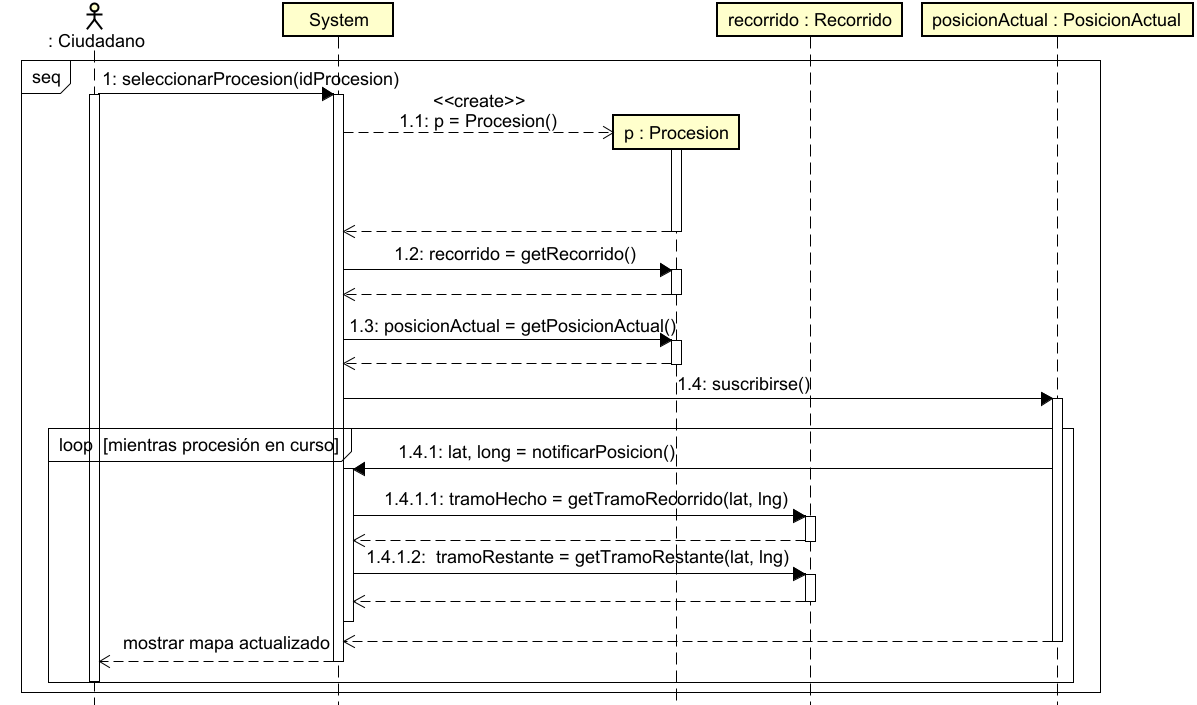
\includegraphics[width=1\textwidth,keepaspectratio]{imagenes/DSCasoUsoVerProcesion.png}
\caption{Diagrama de secuencia del CU ``Visualizar procesión en tiempo real''}
\label{fig:secVisualizarProcesion}
\end{figure}

En el caso de uso \textit{Compartir ubicación durante procesión} (Figura~\ref{fig:secCompartirUbicacion}), el cofrade accede a la procesión activa de su cofradía y activa la opción de compartir su ubicación. El sistema solicita los permisos de localización si no los tiene concedidos: si el cofrade los deniega, se le informa de que no es posible compartir la ubicación sin permiso; si los concede, el sistema comienza a actualizar de forma periódica la posición del cofrade mientras la procesión sigue en curso.

\begin{figure}[H]
\centering
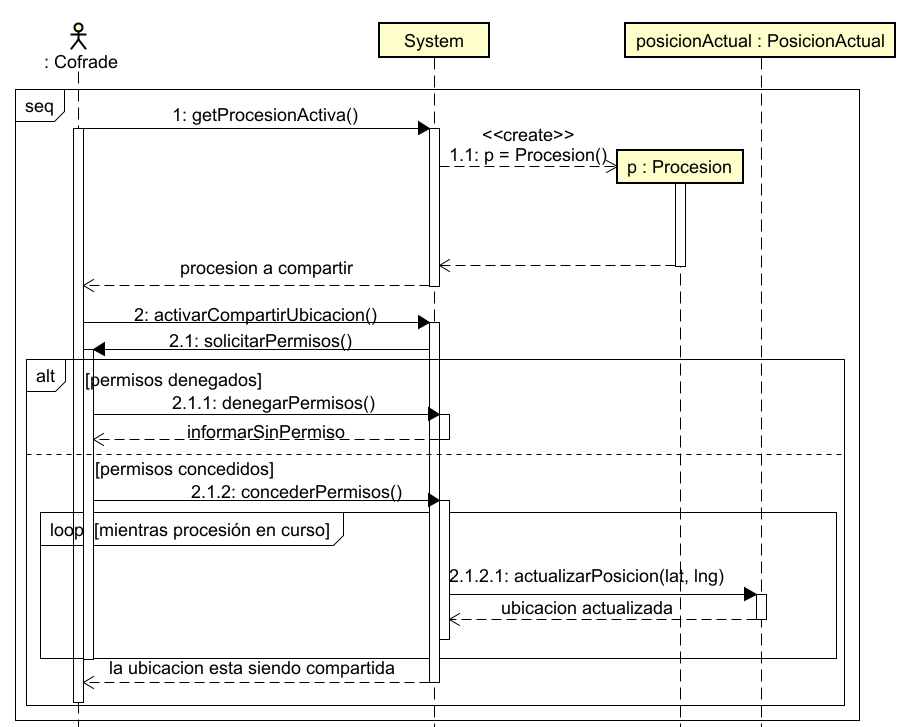
\includegraphics[width=1\textwidth,keepaspectratio]{imagenes/DSCasoUsoCompartirUbi.png}
\caption{Diagrama de secuencia del CU ``Compartir ubicación durante procesión''}
\label{fig:secCompartirUbicacion}
\end{figure}

En el caso de uso \textit{Acceso como cofrade} (Figura~\ref{fig:secAccesoCofrade}), el usuario selecciona la opción de registro y el sistema le muestra el formulario correspondiente. Al introducir el código de acceso de su cofradía, el sistema obtiene el \texttt{CodigoAcceso} correspondiente y lo valida, informando al usuario del acceso correcto o de un error de validación según el resultado.

\begin{figure}[H]
\centering
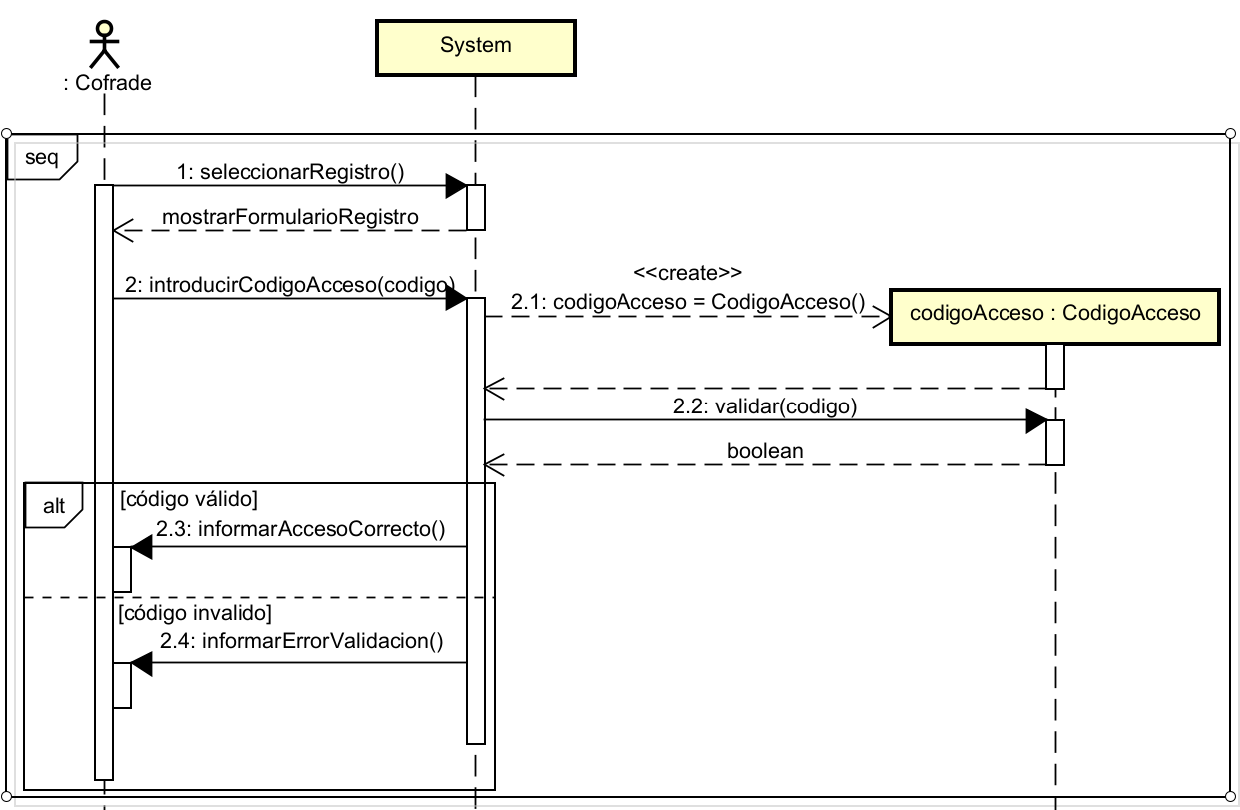
\includegraphics[width=1\textwidth,keepaspectratio]{imagenes/DSCasoUsoAccesoCofrade.png}
\caption{Diagrama de secuencia del CU ``Acceso como cofrade''}
\label{fig:secAccesoCofrade}
\end{figure}

En el caso de uso \textit{Dar de alta ciudad} (Figura~\ref{fig:secAltaCiudad}), el administrador accede al panel de administración, donde el sistema le muestra la lista de ciudades existentes, y selecciona la opción de añadir una nueva ciudad. Tras introducir los datos, el sistema construye la instancia de \texttt{Ciudad} correspondiente y valida los datos introducidos, repitiendo la solicitud hasta que estos son válidos, momento en el que la ciudad queda dada de alta.

\begin{figure}[H]
\centering
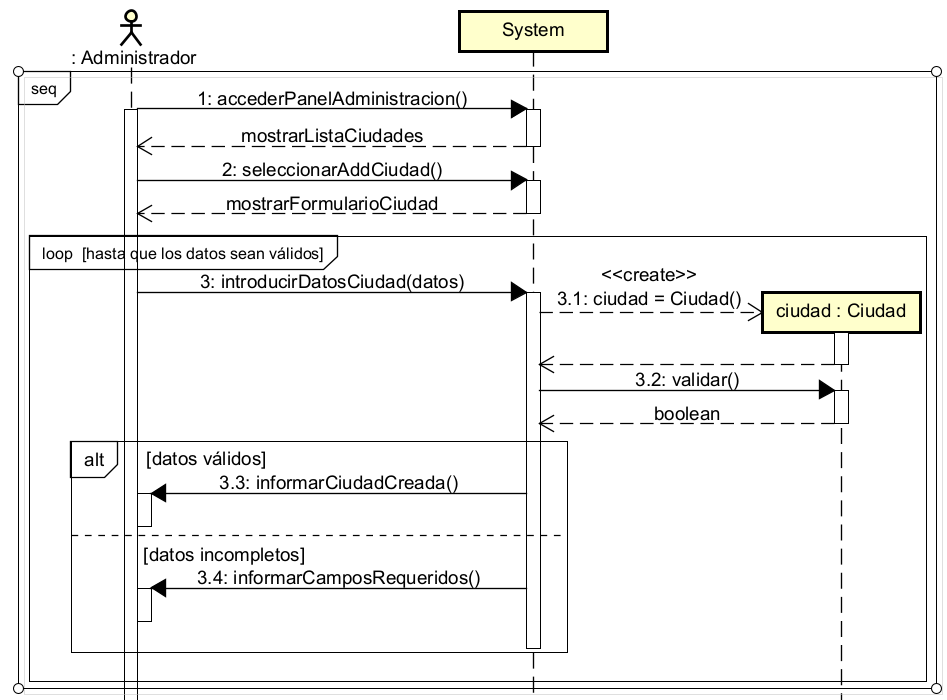
\includegraphics[width=1\textwidth,keepaspectratio]{imagenes/DSCasoUsoCrearCiudad.png}
\caption{Diagrama de secuencia del CU ``Dar de alta ciudad''}
\label{fig:secAltaCiudad}
\end{figure}

% TODO: diagramas de secuencia pendientes de añadir - Editar ciudad, Dar de baja ciudad y Crear alerta.
